% File: jupiter-schedule-c3o3.tex

\documentclass{standalone}
\usepackage{tikz}
\usetikzlibrary{calc, positioning, arrows.meta}

\def\s{s}  % server
\def\b{bot} % literal string
\tikzset{seq/.style = {draw, circle, outer sep = 5pt, inner sep = 2pt, scale = #1, left}}

% send: the sender sends operation to the receiver
\newcommand{\send}[5]{% #1: sender; #2: receiver; #3: sender pos; #4: receiver pos; #5: seq. number;
  \draw[->]  ($(#1)!#3!(#1\b)$) node[seq = 0.60] {#5} to ($(#2)!#4!(#2\b)$) node[seq = 0.60] {$#5$};
}

% csend: client sends operation to the server
\newcommand{\csend}[4]{% #1: client; #2: client pos; #3: server pos; #4: seq. number
  \draw[->]  ($(#1)!#2!(#1\b)$) node[seq = 0.60, fill = purple!40] {#4} to ($(\s)!#3!(\s\b)$) node[seq = 0.50] {$#4$};
  % \send{#1}{\s}{#2}{#3}{#4}
}

% ssend: the server sends operation to client 
\newcommand{\ssend}[4]{% #1: client; #2: server pos; #3: client pos; #4: seq. number
  \draw[->, dashed]  ($(\s)!#2!(\s\b)$) to ($(#1)!#3!(#1\b)$) node[solid, seq = 0.50] {$#4$};
  % \send{\s}{#1}{#2}{#3}{#4}
}

\begin{document}
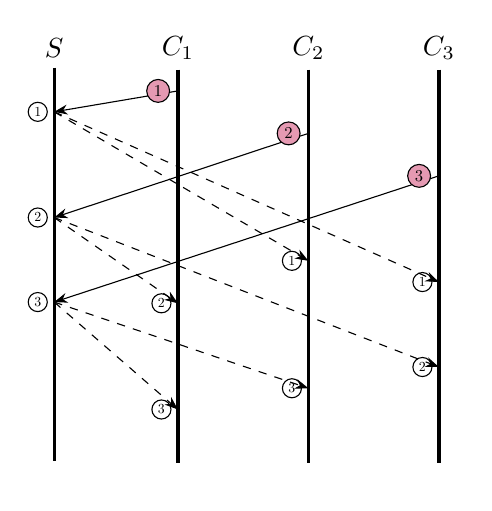
\begin{tikzpicture}[timeline/.style = {very thick}, >=Stealth]
  \node[] (\s) {$S$};
  \node[right = of s] (c1) {$C_1$};
  \node[right = of c1] (c2) {$C_2$};
  \node[right = of c2] (c3) {$C_3$};

  \foreach \r/\rbot in {s/sbot, c1/c1bot, c2/c2bot, c3/c3bot} {
	\node[below = 5.0cm of \r] (\rbot) {};
	\draw[timeline] (\r) to (\rbot);
  }

  % op 1
  \csend{c1}{0.10}{0.15}{1}
  \ssend{c2}{0.15}{0.50}{1}
  \ssend{c3}{0.15}{0.55}{1}

  % op 2
  \csend{c2}{0.20}{0.40}{2}
  \ssend{c1}{0.40}{0.60}{2}
  \ssend{c3}{0.40}{0.75}{2}

  % op 3
  \csend{c3}{0.30}{0.60}{3}
  \ssend{c1}{0.60}{0.85}{3}
  \ssend{c2}{0.60}{0.80}{3}
\end{tikzpicture}
\end{document}
